\documentclass{beamer}
\usepackage[T1]{fontenc}
\usepackage[utf8]{inputenc}
\usepackage{lmodern}
\usepackage[ngerman]{babel}
\usepackage{graphics}
\usepackage{amsmath}
\usetheme{Singapore}
\usecolortheme{dove}
\graphicspath{{images/}{../comics/}}
\newcommand{\hiddencell}[2]{\action<#1->{#2}}
\AtBeginSection[]
{
  \begin{frame}[plain]
    \frametitle{}
    {\footnotesize
      \tableofcontents[currentsection]
    }
  \end{frame}
}

\title{Grundbegriffe der Informatik}
\author{Patrick Niklaus}

\begin{document}
\begin{frame}
  \frametitle{Grundbegriffe der Informatik}
  \framesubtitle{4. Tutorium}
  \begin{description}
    \item \textbf{Name:} Patrick Niklaus
    \item \textbf{E-Mail:} patrick.niklaus@student.kit.edu
    \item \textbf{Nr:} 43
  \end{description}
\end{frame}

\section{Übungsblatt}
\begin{frame}
  \frametitle{Anmerkungen zum letzten Übungsblatt}
  \begin{itemize}
    \item $k_{i+1} \longleftarrow k_i + 1$
    \item Schleifenkopf-Bedingung bei Vollständigen Induktion beachten.
    \item Immer hinschreiben aus welcher Menge eine Variable ist.
  \end{itemize}
\end{frame}

\section{Kontextfreie Grammatiken}
\subsection{Definitionen}
\begin{frame}
  \frametitle{Kontextfreie Grammatiken}
  \begin{definition}
    Seien folgende Mengen gegeben:
    \begin{description}
      \item[N:] Menge von Nichtterminalsymbolen
      \item[T:] Menge von Terminalsymbolen
      \item[S:] $S \in N$ Startsymbol
      \item[$P \subset N \times V^*$:] Menge von Produktionen, \\
      $V := (N \cup T)$
    \end{description}
    Dann heißt der Tupel G := (N, T, S, P) \emph{kontextfreie Grammatik}.
  \end{definition}\pause
  Schreibweisen:
  \begin{itemize}
    \item Anstelle von $(a, b) \in P$ schreibt man $a \longrightarrow b$.
    \item Die Sprache die von G erzeugt wird nennt man L(G).
  \end{itemize}
\end{frame}

\begin{frame}
  \frametitle{Beispiele}
  \begin{exampleblock}{Beispiele}
    \begin{itemize}
      \item $G_1 := (\{X\}, \{a, b\}, X, \{X \longrightarrow aXb | \varepsilon\})$
      \item $G_2 := (\{X, Y, Z\}, \{0, 1\}, X, \{X \longrightarrow 0Y | 1Z, Y \longrightarrow 0Y|\varepsilon, Z \longrightarrow 1Z|\varepsilon\})$
       \item $G_3 := (\{X\}, \{0\}, X, \{X \longrightarrow X | \varepsilon\})$
    \end{itemize}
  \end{exampleblock}
\end{frame}

\subsection{Aufgaben}
\begin{frame}
  \frametitle{Fragen}
  \begin{exampleblock}{}
    \begin{enumerate}
      \item Gibt es Grammatiken für die gilt: $L(G) = \{\}$?
      \item Welche Sprache erzeugt: $G_1 := (\{X\}, \{0\}, X, \{X \longrightarrow X\})$
      \item Ist $G_2 := (\{X\}, \{a, b\}, a, \{X \longrightarrow \varepsilon\})$ eine gültige Grammatik?
    \end{enumerate}
  \end{exampleblock}
\end{frame}
\begin{frame}
  \frametitle{Aufgaben}
  \begin{exampleblock}{In Mengen M aus Studenten mit $|M| \leq 3$}
    Welche Sprachen erzeuge folgende Grammatiken.
    \begin{enumerate}
      \item $G_1 := (\{X, Y\}, \{a, b\}, X, \{X \longrightarrow aY | \varepsilon, Y \longrightarrow bX\})$
      \item $G_2 := (\{X, Y, Z\}, \{a, b, c\}, X,$\\
             $\{X \longrightarrow Ya | Yb | Yc, Y \longrightarrow ZZY | \varepsilon, Z \longrightarrow a | b | c\})$
    \end{enumerate}
    Gebt eine jeweils Grammatik an für die gilt $L(G) = L_i$:
    \begin{enumerate}
      \item $L_1 := \{ab, cd\}^* \cdot \{a, c\}^2$
      \item $A := \{0, 1\}$, $L_2 := \{w  \in A^*| Num_0(w) = Num_1(w)\}$
    \end{enumerate}
  \end{exampleblock}
\end{frame}
\begin{frame}
  \frametitle{Bonus-Aufgabe}
  \begin{exampleblock}{In Mengen M aus Studenten mit $|M| \leq 3$}
    Konstruiert eine Grammatik die alle E-Mail-Adresse aus den Buchstaben {a, b, c} erzeugt.
    \emph{Hinweis}: $T := \{a, b, c, @, ., \_\}$
  \end{exampleblock}\pause
  \begin{exampleblock}{Lösung}
    $G = (N, T, S, P)$
    \begin{itemize}
      \item $N = \{E, A, B\}$
      \item $T = \{a, b, c, ., \_\}$
      \item $S = E$
      \item $P = \{E \longrightarrow A@B.B, A \longrightarrow B|\_A, B \longrightarrow aB | bB | cB | \varepsilon\}$
    \end{itemize}
  \end{exampleblock}
\end{frame}
\section{Relationen}
\subsection{Motivation}
\begin{frame}
	\frametitle{Motivation Relationen}
	\begin{alertblock}{Anschaulich}
		Durch Relationen werden Elemente einer oder mehrerer Mengen in Beziehung zueinander gesetzt:
	\end{alertblock}\pause
  \begin{exampleblock}{Beispiele}
		\begin{itemize}
			\item Ford ist mit Arthur, Zap und Trillian befreundet.
      \item 4 ist kleiner als 5, 3 ist kleiner als 13, ...
		\end{itemize}
  \end{exampleblock}\pause
	\begin{block}{Wozu brauchen wir das?}
		Relationen werden zur Modellierung von Systemen benötigt: \pause
		\begin{itemize}
			\item Relationen sind Grundlage der verschiedenen Diagramme der UML.
			\item Graphen sind graphische Darstellungen von Relationen.
		\end{itemize}
	\end{block}
\end{frame}

\subsection{Definitionen}
\begin{frame}
  \frametitle{Relation}
  \begin{definition}
    \begin{itemize}
      \item Seien A, B zwei Mengen. $ R \subseteq A \times B $
      \item R ist eine Teilmenge des Kreuzproduktes zweier Mengen und heißt \emph{Relation}.
      \item Man schreibt auch: xRy für $(x, y) \in R$
      \item Ist A = B so nennt man R auch eine \emph{homogene} Relation.
    \end{itemize}
  \end{definition}
\end{frame}

\begin{frame}
	\frametitle{Produkt von Relationen}
	\begin{definition}
		Sind $R \subseteq M_1 \times M_2$ und $S \subseteq M_2 \times M_3$ zwei Relationen.\\
    \begin{itemize}
			\item $S \circ R = \{(x,z) \in M_1 \times M_3 \mid \exists y \in M_2 : (x,y) \in R \wedge (y,z) \in S \}$ heißt das \emph{Produkt der Relationen S und R}.
			\item $Id_M = \{(x,x) \mid x \in M \}$ heißt die \emph{identische Abbildung}
    \end{itemize}
	\end{definition}
\end{frame}

\begin{frame}
	\frametitle{Potenz von Relationen}
  \begin{definition}
		Sei $R \subseteq M \times M$ eine \emph{homogene} Relation.
    $R^i$ heißt die {\em i-te Potenz} von R und ist definiert als:
    \begin{itemize}
			\item $R^0=Id_M$
			\item $\forall i \in \mathbb N_0: R^{i+1}=R \circ R^i$
    \end{itemize}
	\end{definition}
\end{frame}

\begin{frame}
	\frametitle{Äquivalenzrelation}
	\begin{definition}
    Sei R eine homogene Relation über M. $x, y, z \in M$.\\
    Hat R folgende Eigenschaften:
		\begin{description}
			\item[reflexiv] $x R x$
			\item[transitiv] $x R y \wedge y R z \Rightarrow x R z$
			\item[symmetrisch] $x R y \Rightarrow y R x$
		\end{description}
		So heißt R eine \emph{Äquivalenzrelation}.
	\end{definition}
\end{frame}

\subsection{Reflexiv-transitive Hülle}
\begin{frame}
	\frametitle{Reflexiv-Transitive Hülle}
	\begin{definition}
    Sei R eine Relation.\\
		$R^* = \bigcup \limits_{i=0}^{\infty} R^i$\\
		$R^*$ heißt die \emph{reflexiv-transitive Hülle} von R.
	\end{definition} \pause
  \begin{alertblock}{Anschaulich}
		Sie ist die Erweiterung der Relation um die Paare, die notwendig sind um Reflexivität und Transitivität herzustellen.
  \end{alertblock}
\end{frame}

\begin{frame}
	\frametitle{Facebook Freundschaften}
	\begin{exampleblock}{}
    {\small
			Sei $M = \{ Gertrud, Holger, Lars, Katja, Martin, Nina \}$ eine Menge von Nutzern.\\
			$R \subseteq M \times M $ sei die "`ist-befreundet-mit"'-Relation.
		\begin{itemize}
			\item $R = \{ (Martin,Holger), (Lars,Katja), (Nina,Holger),$ \\
						$(Gertrud,Holger), (Katja, Nina) \} \bigcup \{${dazu sym. Tupel}$\}$ \pause
			\item $R^0=\{ (Martin,Martin), ..., (Holger,Holger) \}$ \pause
			\item $R^1=R$ "'Freundschaft 1. Grades."' \pause
			\item $R^2=\{ (Martin,Nina), (Martin,Gertrud), (Martin,Martin),$ \\
						$(Lars,Nina), (Lars,Lars), (Nina,Gertrud),(Nina,Martin),$ \\
						$(Nina,Nina), (Nina,Lars), (Katja,Katja), (Katja,Holger), $ \\
						$(Gertrud,Gertrud), (Gertrud,Martin), (Gertrud,Nina), $ \\
						$(Holger,Holger), (Holger,Katja)\}$ "'Freundschaft 2. Grades"' \pause
			\item $R^*=?$ "'Gibt es eine Verbindung durch Freunde beliebigen Grades?"'
			%\item wegen Symmetrie und Unsinnigkeit der Reflexivität, entfällt Einiges % Funktionen sind kommutativ, Relationen symmetrisch
		\end{itemize}
    }
	\end{exampleblock}
\end{frame}

\subsection{Aufgaben}
\begin{frame}
	\frametitle{Aufgaben}
  \begin{exampleblock}{}
    Bestimmt die reflexiv-transitive Hülle der Relationen.\\
    $M := \{1, 2, 3, 4\}, R_i \subset M \times M$
    \begin{enumerate}
      \item $R_1 := \{(1, 2), (1, 4), (2, 3)\}$
      \item $R_2 := \{(1, 1), (2, 2)\}$
      \item $R_3 := \{(1, 2), (3, 4), (4, 2)\}$
    \end{enumerate}
  \end{exampleblock}\pause
  \begin{exampleblock}{Lösungen}
    \begin{enumerate}
      \item $R_1^* := \{(1, 1), (1, 2), (1, 3), (1, 4), (2, 2), (2, 3), (3, 3), (4, 4)\}$
      \item $R_2^* := \{(1, 1), (2, 2), (3, 3), (4, 4)\}$
      \item $R_3^* := \{(1, 1), (1, 2), (2, 2), (3, 2), (3, 3), (3, 4), (4, 2), (4, 4)\}$
    \end{enumerate}
  \end{exampleblock}
\end{frame}


\section{Abschluss}
\subsection{Zusammenfassung}
\begin{frame}
  \frametitle{Was ihr mitnehmen sollt}
  \begin{enumerate}
    \item bla
  \end{enumerate}
\end{frame}

\subsection{xkcd}
\begin{frame}[plain]
  \begin{figure}
    \begin{center}
      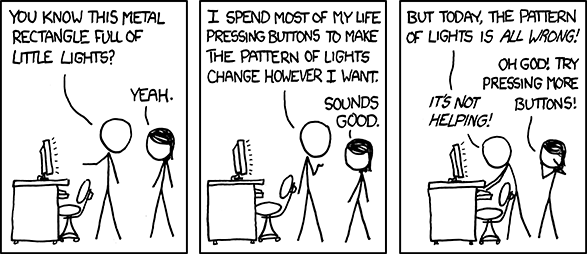
\includegraphics[width=320pt]{computer_problems}
    \end{center}
  \end{figure}
\end{frame}

\end{document}
